Here we prove that the \emph{Core Structural Connectivity Network problem}, called \PROBLEM, is NP-complete. In our reduction, we use the \emph{Steiner Tree problem}~\cite{Garey1979}, called \STEINER~in the
following. Given an edge-weighted graph $G' = (V',E',w)$, a subset
$S \subseteq V'$ of nodes, and a real $k \geq 0$, \STEINER~consists in
determining if there exists a connected subgraph $H$ such that $S \subseteq V(H)$ and $\sum_{e \in E(H)}{w(e)} \leq k$.
The decision version of \STEINER~is NP-complete even if all weights are equal~\cite{Garey1979}.

\smallskip

\textbf{Instance of \STEINER.}
Consider any edge-weighted graph $G' = (V',E',w)$ such that $w(e) =
\frac{1}{2}$ for every $e \in E'$.
Given $k \geq 0$, \STEINER~consists in determining if there exists a
connected subgraph $H$ such that $S \subseteq V(H)$ and $|E(S)| \leq
2k$.
Without loss of generality, we assume that $|E'| \geq 2k$ and that
$G'$ is connected.

\smallskip

\textbf{Reduction.}
We construct the instance of \PROBLEM~as follows.
Let $s = |S|$ and let $t \geq 1$ be any positive integer.
Let $G = (V,E,w^{*})$ defined as follows.
Let $V = V' \cup \{v_{i,j} \mid 1 \leq i \leq s, 1 \leq j \leq t\}$
and $E = V \times V$.
Let $S = \{u_{1}, \ldots, u_{s}\}$.
For every $i,j$, $1 \leq i \leq s$, $1 \leq j \leq t$,
$w^{*}_{v_{i,j},u_{i}} = 1$ and $w^{*}_{v_{i,j},u} = 0$ for every $u
\in V \setminus \{u_{i}\}$.
Furthermore, for every $e \in E'$, set $w^*(e) = w(e) =
\frac{1}{2}$, and for every $u,u' \in V'$ such that $\{u,u'\} \notin
E'$, then set $w^*_{e} = 0$.
Finally, we set $A = \frac{s.t+k}{s.t+2k}$ and $B =
\frac{\frac{1}{2}(|E'|-2k)}{s.t+2k}$.


\begin{lemma}
\label{lem:beta}
If $|E^*| < s.t+2k$, then any solution for \PROBLEM~is not
admissible because $\beta(w^{*},E^*) > B$.
\end{lemma}

\begin{proof}
Suppose that $|E^*| < s.t+2k$.
In order to minimize $\sum_{e \in E \setminus E^*} w^*(e)$,
$E^*$ must contain $\{\{v_{i,j},u_{i}\} \mid 1 \leq i \leq s, 1 \leq
j \leq t\}$ if $|E^*| \geq s.t$.
(Otherwise we select a subset of this set of edges.)
Indeed, by construction of $G$, we have $w^{*}_{v_{i,j},u_{i}} = 1$
for every $i,j$, $1 \leq i \leq s$, $1 \leq j \leq t$.
Then, if $|E^*| - s.t > 0$, $E^*$ must contain $|E^*| - s.t$
edges of $E'$, that is edges of $E$ of weight $\frac{1}{2}$ each.
Recall that there are exactly $s.t$ edges of weight $1$, and the other
edges have weight $0$ or $\frac{1}{2}$.

There are two cases.
First, suppose that $|E^*| \geq s.t$.
We get that $\sum_{e \in E \setminus E^*} w^*(e) =
\frac{1}{2}(|E'| - (|E^*| - s.t))$.
Since $|E^*| - s.t < 2k$, then we get that $\sum_{e \in E \setminus E^*} w^*(e) =
\frac{1}{2}(|E'| - (|E^*| - s.t)) > \frac{1}{2}(|E'| - 2k)$.
Furthermore, since $|E^*| < s.t+2k$, we get that 
$\frac{\frac{1}{2}(|E'| - (|E^*| - s.t))}{|E^*|} >
\frac{\frac{1}{2}(|E'|-2k)}{s.t+2k}$.
Thus, we proved that $\beta(w^{*},E^*) = \frac{\sum_{e \in E \setminus E^*}
  w^*(e)}{|E^*|} > B$.

Second, suppose that $|E^*| < s.t$.
We get that $\sum_{e \in E \setminus E^*} w^*(e) = s.t - |E^*|
+ \frac{|E'|}{2}$.
Since $s.t - |E^*| + \frac{|E'|}{2} > \frac{1}{2}(|E'| - (|E^*| -
s.t))$, we obtain the result by the arguments described for the first
case.

Finally, if $|E^*| < s.t+2k$, then there is no admissible solution
for \PROBLEM.
\end{proof}

\begin{lemma}
\label{lem:alpha}
If $|E^*| > s.t+2k$, then any solution for \PROBLEM~is not
admissible because $\alpha(w^{*},E^*) < A$.
\end{lemma}

\begin{proof}
  Suppose that $|E^*| > s.t+2k$.
  In order to maximize $\sum_{e \in E^*} w^*(e)$,
$E^*$ must contain $\{\{v_{i,j},u_{i}\} \mid 1 \leq i \leq s, 1 \leq
  j \leq t\}$ and $|E^*| - s.t$ edges of $E'$.
Indeed, by construction of $G$, we have $w^{*}_{v_{i,j},u_{i}} = 1$
for every $i,j$, $1 \leq i \leq s$, $1 \leq j \leq t$.
Furthermore, $w^*(e) = \frac{1}{2}$ for every $e \in E'$.
Recall that there are exactly $s.t$ edges of weight $1$, and the other
edges have weight $0$ or $\frac{1}{2}$.
We get that $\alpha(w^{*},E^*) = \frac{s.t + \frac{1}{2}(|E^*| -
  s.t)}{|E^*|} < \frac{s.t+k}{s.t+2k} = A$.
Indeed, the average weight is lower when there are more edges of
weight $\frac{1}{2}$ (the number of edges of weight $1$ is the same in
both ratios).

Finally, if $|E^*| > s.t+2k$, then there is no admissible solution
for \PROBLEM.
\end{proof}

By Lemma~\ref{lem:beta} and Lemma~\ref{lem:alpha}, we get the
following corollary.

\begin{corollary}
\label{cor:alpha-beta}
Any solution for \PROBLEM~is such that $|E^*| = s.t + 2k$.
\end{corollary}

We prove in Lemma~\ref{lem:droite-gauche} and in
Lemma~\ref{lem:gauche-droite} that there is an admissible solution for
\PROBLEM~if and only if there is an admissible solution for \STEINER.

\begin{lemma}
\label{lem:droite-gauche}
If there is an admissible solution for \STEINER, then there is an
admissible solution for \PROBLEM.
\end{lemma}

\begin{proof}
Suppose there is an admissible solution for \STEINER.
We prove that there is an admissible solution for \PROBLEM.
Let $H$ be a connected subgraph such that $S
\subseteq V(H)$ and $\sum_{e \in E(H)}{w(e)} = \frac{1}{2}|E(|H)|
\leq k$.
If $|E(H)| = 2k$, then set $E^* = E(H) \cup \{\{v_{i,j},u_{i}\} \mid 1 \leq i \leq s, 1 \leq j \leq
t\}$.
If $|E(H)| < 2k$, then set $E^* = E(H) \cup \{\{v_{i,j},u_{i}\} \mid 1 \leq i \leq s, 1 \leq j \leq
t\} \cup F$, where $F \subseteq E'$ such that $F \neq E(H) =
\emptyset$, $w^*(e) = \frac{1}{2}$ for every $e \in F$, and such
that the graph induced by $E(H) \cup F$ is connected.
The last condition comes from Corollary~\ref{cor:alpha-beta} in order
to get the right number of edges in $E^*$.
This condition is always possible to satisfy because $G'$ is
connected.

The graph induced by $E^*$ is connected.
Indeed, $H$ is an admissible solution for \STEINER, $E(H) \cup F$ is
connected by construction, and $\{\{v_{i,j},u_{i}\} \mid 1 \leq j \leq
t\}$ is a set of edges all adjacent to $u_{i} \in S$ for every $i$, $1
\leq i \leq s$.

Furthermore, we get
$$\alpha(w^{*},E^*) = \frac{\sum_{e \in E^*}
  w^*(e)}{|E^*|} = \frac{s.t+k}{s.t+2k} = A$$
and
$$\beta(w^{*},E^*) = \frac{\sum_{e \in E \setminus E^*}
  w^*(e)}{|E^*|} = \frac{\frac{1}{2}(|E'|-2k)}{s.t+2k} = B.$$

Finally, we proved that there is an admissible solution for \PROBLEM.
\end{proof}


\begin{lemma}
\label{lem:gauche-droite}
If there is an admissible solution for \PROBLEM, then there is an
admissible solution for \STEINER.
\end{lemma}

\begin{proof}
Suppose there is an admissible solution for \PROBLEM.
We prove that there is an admissible solution for \STEINER.
Let $E^* \subseteq E$ be such that the graph induced by $E^*$ is
connected, and such that $\alpha(w^{*},E^*) \geq
\frac{s.t+k}{s.t+2k} = A$ and $\beta(w^{*},E^*) \leq =
\frac{\frac{1}{2}(|E'|-2k)}{s.t+2k} = B$.

We first prove that $\{\{v_{i,j},u_{i}\} \mid 1 \leq i \leq s, 1 \leq j \leq
t\} \subseteq E^*$.
By Corollary~\ref{cor:alpha-beta}, we know that $|E^*| = s.t + 2k$.
Thus, it necessarily means that $\sum_{e \in E^*} w^*(e) \geq s.t
+ k$.
By construction of $G$, the set of edges of weight $1$ is $\{\{v_{i,j},u_{i}\} \mid 1 \leq i \leq s, 1 \leq j \leq
t\}$, that is $\{e \in E \mid w^*(e) > \frac{1}{2}\} =
\{\{v_{i,j},u_{i}\} \mid 1 \leq i \leq s, 1 \leq j \leq t\}$.
We get that $\{\{v_{i,j},u_{i}\} \mid 1 \leq i \leq s, 1 \leq j \leq
t\} \subseteq E^*$ because, otherwise, we would have $\sum_{e \in E^*} w^*(e) < s.t
+ k$.

Furthermore, every $e \in E^* \cap E'$ is such that
$w^*(e) = \frac{1}{2}$.
Indeed, otherwise, we would have $\sum_{e \in E^*} w^*(e) < s.t
+ k$.

Finally, since $E^*$ is an admissible solution for \PROBLEM,
then it means that the graph induced by the set of edges $E^* \cap
E'$ is connected and is such that for every $u_{i}$, $1 \leq i \leq
s$, then there is an edge $e \in E^* \cap E'$ that is adjacent to
$u_{i}$.
By the previous remark, every edge in $E^* \cap E'$ has weight
$\frac{1}{2}$.
Thus, it means that there is $E^* \cap E'$ is an admissible solution
for \STEINER~considering the graph $G'$.
Indeed $|E^* \cap E'| = 2k$ and so $\sum_{e \in E^* \cap E'}w(e)
= k$.
\end{proof}



We are now able to prove the NP-completeness of \PROBLEM.

\begin{theorem}
\label{the:NP-complete-with-Steiner}
\PROBLEM~is NP-complete.
\end{theorem}
\begin{proof}
The reduction is clearly polynomial.
Furthermore, Lemma~\ref{lem:droite-gauche} and
Lemma~\ref{lem:gauche-droite} prove the equivalence between
\PROBLEM~and \STEINER.
Since the decision version of \STEINER~is NP-complete even if all weights are
equal~\cite{Garey1979}, then we obtain the NP-completeness of the
decision version of \PROBLEM.
\end{proof}

%As an illustration of the proof of Theorem~\ref{the:NP-complete-with-Steiner}, consider the instance of \STEINER~and \PROBLEM~depicted in Figure~\ref{fig:np}. In this example, we set $s = 5$, $t = 3$, $k = 3$. The edges of $E'$ have weight $\frac{1}{2}$, the edges of $E$ have weight $1$, and the other edges (non-edges in Figure~\ref{fig:np}) have weight $0$. We set $A = \frac{6}{7}$ and $B = \frac{1}{3}$. There is an admissible solution for \PROBLEM~with $|E^*| = 21$ and so an admissible solution for \STEINER~with $|E(H)| = 6$. We get $\alpha(w^{*},E^*) = A$ and $\beta(w^{*},E^*) = B$.

%\begin{figure}[t]
%\centering
%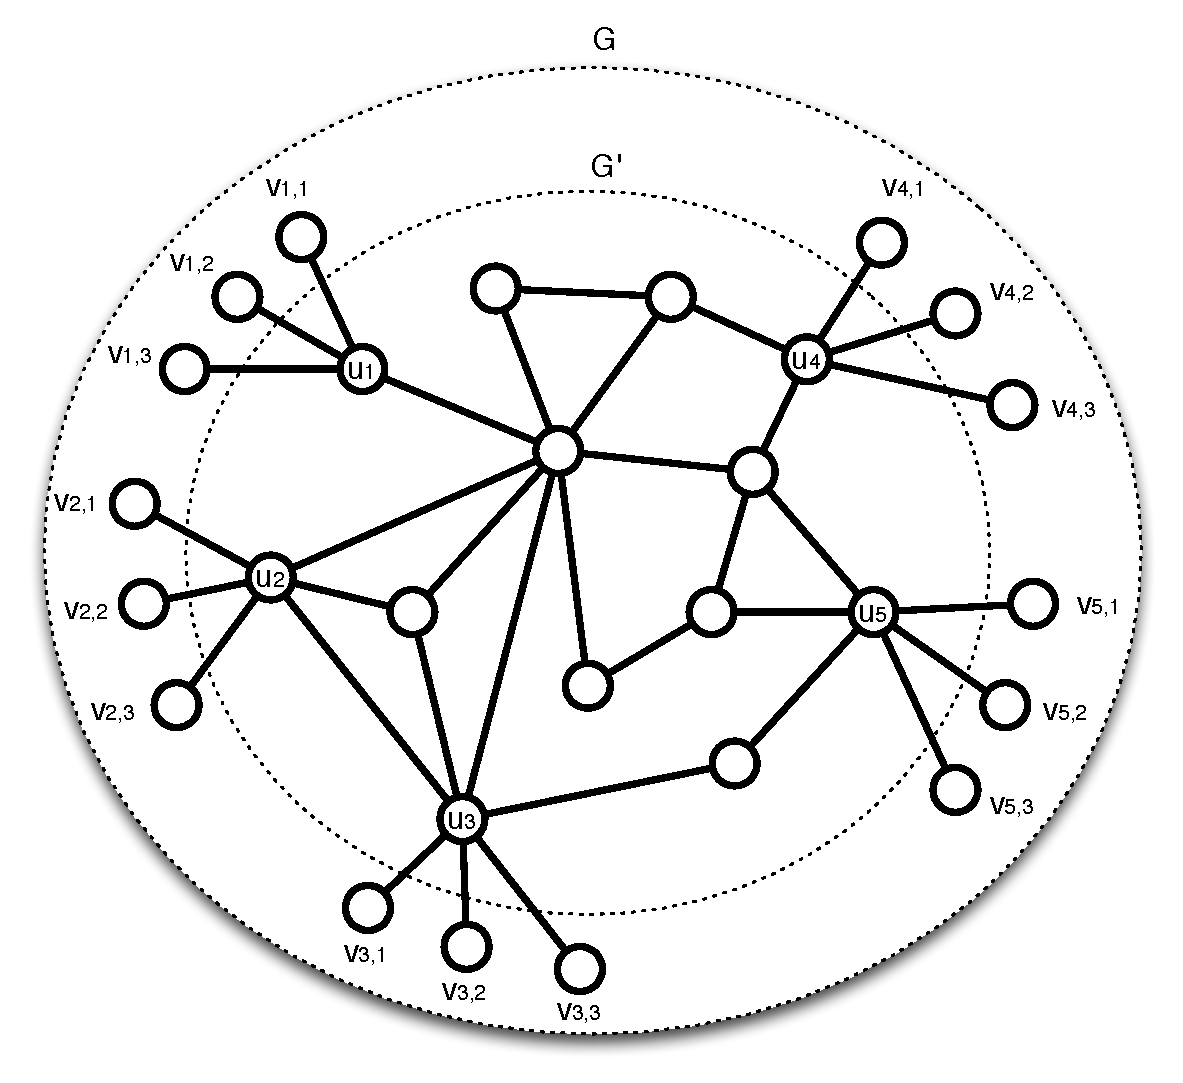
\includegraphics[width=0.5\textwidth]{np-complete-2.pdf}
%\caption{Illustration of the proof of
%  Theorem~\ref{the:NP-complete-with-Steiner}}
%\label{fig:np}
%\end{figure}

